\begin{figure}[h]
	\centering
	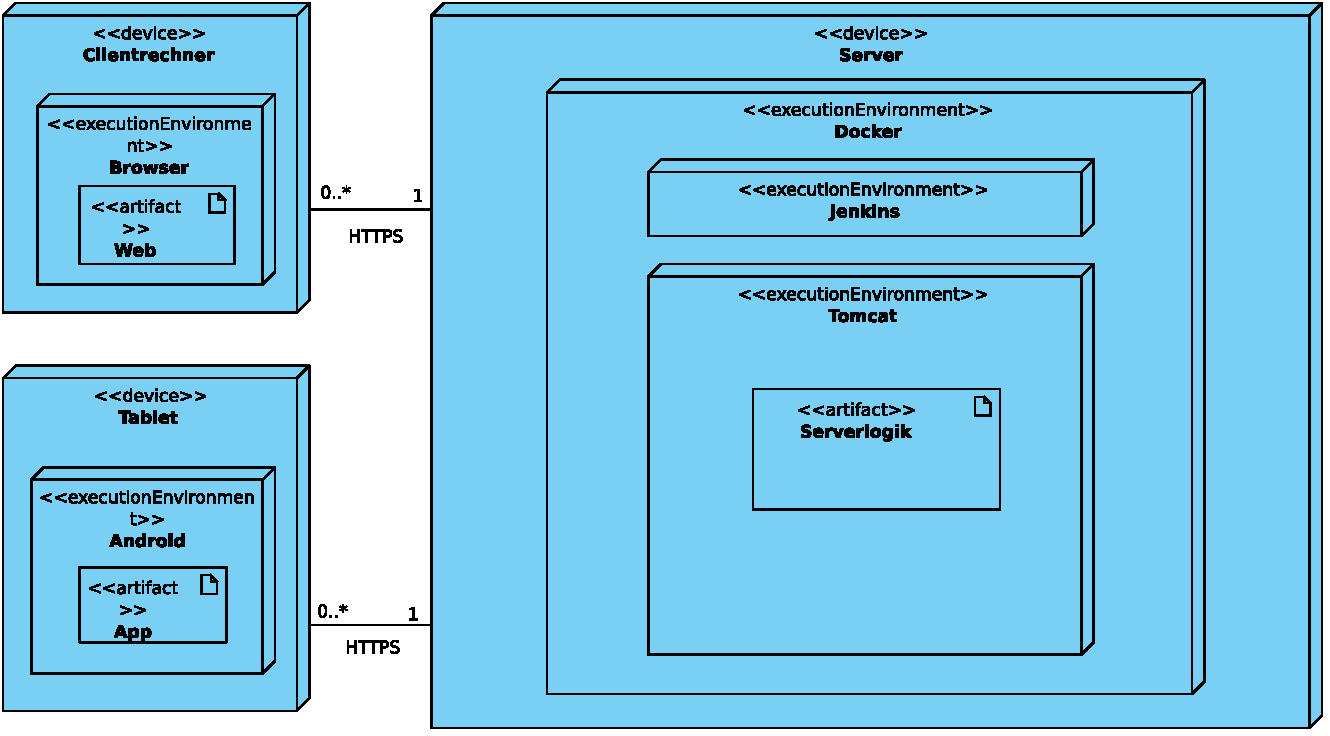
\includegraphics[width=\textwidth]{img/Diagramme/Verteilung}		
	\caption{Verteilungsdiagramm}
	\label{fig:verteilungsdiagramm}
\end{figure}
\noindent
Die App-Komponente läuft auf einem Tablet Android 6.0 oder höher, während 
die Web-Komponente  in den Browsern auf dem Rechnern des Nutzers läuft.
Die Geschäftslogik in der Komponente Serverlogik wird auf einem physikalischen Server ausgeführt, auf dem in einem Docker-Image neben Apache Tomcat auch Jenkins betrieben wird.
Sowohl die Clientrechner als auch die Tablets sind mit dem Server über HTTPS verbunden.

\newpage
\section{REST Schnitstelle}
\begin{table}[htbp]
\centering
\begin{tabularx}{\linewidth+20pt}{|X|l|X|}
\hline
\rowcolor[HTML]{C0C0C0}
\textbf{Aktion} & \textbf{HTTP Methode} & \textbf{Endpunkt}\\
\rowcolor[HTML]{E7E7E7}
createService(s) & POST & /services\\
editService & PUT & /services/\{service\(_{\text{id}}\)\}\\
\rowcolor[HTML]{E7E7E7}
getServices & GET & /services\\
getServiceDetails & GET & /services/\{service\(_{\text{id}}\)\}\\
\rowcolor[HTML]{E7E7E7}
deleteService & DELETE & /services/\{service\(_{\text{id}}\)\}\\
\hline
checkCompatibility & GET & /services/\{user\(_{\text{id}}\)\(_{\text{1}}\)\}/\{user\(_{\text{id}}\)\(_{\text{2}}\)\}\\
\hline
\rowcolor[HTML]{E7E7E7}
getCompositions & GET & /compositions\\
getCompositionDetail & GET & /compositions/\{comp\(_{\text{id}}\)\}\\
\rowcolor[HTML]{E7E7E7}
createComposition & POST & /compositions\\
editComposition & PUT & /compositions/\{comp\(_{\text{id}}\)\}\\
\rowcolor[HTML]{E7E7E7}
\hline
getUserPermissions & GET & /compositions/\{comp\(_{\text{id}}\)\}/users\\
createUserPermission & POST & /compositions/\{comp\(_{\text{id}}\)\}/users/\{email\}\\
\rowcolor[HTML]{E7E7E7}
editUserPermission & PUT & /compositions/\{comp\(_{\text{id}}\)\}/users/\{email\}\\
deleteUserPermission & DELETE & /compositions/\{comp\(_{\text{id}}\)\}/users/\{user\(_{\text{id}}\)\}\\
\rowcolor[HTML]{E7E7E7}
\hline
getUsers & GET & /users\\
getUserDetails & GET & /users/\{user\(_{\text{id}}\)\}\\
\rowcolor[HTML]{E7E7E7}
editUser & PUT & /users/\{user\(_{\text{id}}\)\}\\
register & POST & /users\\
\hline
\end{tabularx}
\caption{Art der Anfrage und zu kontaktierender Endpunkt der API}
\end{table}
\label{sec:org9044419}
\begin{table}[htbp]
\centering
\begin{tabularx}{\linewidth+20pt}{|X|l|X|}
\hline
\rowcolor[HTML]{C0C0C0}
\textbf{Aktion} & \textbf{Inhalt der Anfrage} & \textbf{erwartete Antwort} \\
\rowcolor[HTML]{E7E7E7}
createService(s) & List of services & 201 - CREATED\\
editService & single service & 200 - OK\\
\rowcolor[HTML]{E7E7E7}
getServices & query: string & 200 - OK + List of \emph{Service}\\
getServiceDetails & - & 200 - OK + \emph{Service}\\
\rowcolor[HTML]{E7E7E7}
deleteService & - & 200 - OK\\
\hline
checkCompatibility & - & 200 - OK + \emph{CompatibilityAnswer}\\
\hline
\rowcolor[HTML]{E7E7E7}
getCompositions & - & 200 - OK + List of \emph{SimpleComp}\\
getCompositionDetail & - & 200 - OK + \emph{DetailComp}\\
\rowcolor[HTML]{E7E7E7}
createComposition & name: string & 201 - CREATED\\
editComposition & \emph{Composition Object} & 200 - OK\\
\rowcolor[HTML]{E7E7E7}
\hline
getUserPermissions & \emph{userAuthorizations} & 200 - OK + List of \emph{SimpleUser}\\
createUserPermission & \emph{userPermission Object} & 201 - CREATED\\
\rowcolor[HTML]{E7E7E7}
editUserPermission & \emph{userPermission Object} & 200 - OK\\
deleteUserPermission & - & 200 - OK\\
\rowcolor[HTML]{E7E7E7}
\hline
getUsers & query: string & 200 - OK + List of \emph{SimpleUser}\\
getUserDetails & - & 200 - OK + \emph{DetailUser}\\
\rowcolor[HTML]{E7E7E7}
editUser & \emph{Detail User} & 200 - OK\\
register & \emph{User} & 201 - CREATED\\
\hline
\end{tabularx}
\caption{Argumente und erwartete Rückgabe eine API Anfrage}
\end{table}